% \iffalse
\let\negmedspace\undefined
\let\negthickspace\undefined
\documentclass[journal,12pt,twocolumn]{IEEEtran}
\usepackage{cite}
\usepackage{amsmath,amssymb,amsfonts,amsthm}
\usepackage{algorithmic}
\usepackage{graphicx}
\usepackage{textcomp}
\usepackage{xcolor}
\usepackage{txfonts}
\usepackage{listings}
\usepackage{enumitem}
\usepackage{mathtools}
\usepackage{gensymb}
\usepackage{comment}
\usepackage[breaklinks=true]{hyperref}
\usepackage{tkz-euclide} 
\usepackage{listings}
\usepackage{gvv}                                        
\def\inputGnumericTable{}                                
\usepackage[latin1]{inputenc}                            
\usepackage{color}                                       
\usepackage{array}                                       
\usepackage{longtable}                                   
\usepackage{calc}                                        
\usepackage{multirow}                                    
\usepackage{hhline}                                      
\usepackage{ifthen}                                      
\usepackage{lscape}
\usepackage{amsmath}
\newtheorem{theorem}{Theorem}[section]
\newtheorem{problem}{Problem}
\newtheorem{proposition}{Proposition}[section]
\newtheorem{lemma}{Lemma}[section]
\newtheorem{corollary}[theorem]{Corollary}
\newtheorem{example}{Example}[section]
\newtheorem{definition}[problem]{Definition}
\newcommand{\BEQA}{\begin{eqnarray}}
\newcommand{\EEQA}{\end{eqnarray}}
\newcommand{\define}{\stackrel{\triangle}{=}}
\theoremstyle{remark}
\newtheorem{rem}{Remark}

\begin{document}

\bibliographystyle{IEEEtran}
\vspace{3cm}

\title{NCERT Mathematics Ex 9.4 Q6}
\author{EE23BTECH11059 - Tejas$^{}$% <-this % stops a space
}
\maketitle
\newpage
\textbf{Question:}
1) Find the sum to n terms of\\$3 \times 8 + 6 \times 11 + 9 \times 14 + ...$
        

    
    \solution
        
        Writing the general term of the series
        \begin{align}
            &x_n=(3r+3)\times(8+3r) \notag \\
            S_n&=\sum_{r=0}^{n}9r^2+33r+24 
        \end{align}
        Using formulas for the sum of n terms (i) and sum of the squares of the n terms (ii) \\
          \begin{align}
            \sum_{r=0}^{n}r&=\frac{n(n+1)}{2} \hspace{2cm}(i)\notag \\
            \sum_{r=0}^{n}r^2&=\frac{n(n+1)(2n+1)}{6} \hspace{2cm}(ii)\notag 
        \end{align}
        
        
        Equation (1) evaluates to
        \\
             \begin{align*}
                S_n=\frac{33n(n+1)}{2} + \frac{9n(n+1)(2n+1)}{6} + 24n
            \end{align*}
        \\
        $Z$ transform of $x_n$:
        \begin{align*}
            X(Z) &= \sum_{n=0}^{\infty} (3n+3)(3n+8)Z^{-n} \\
            X(Z) &= \sum_{n=0}^{\infty} (9n^2 +33n+24)Z^{-n} \\
            %X(Z) = 9(0(Z^{-0})+1(Z^{-1})+4(Z)^{-2}....) + 33(0(Z)^{-0} +1(Z)^-%^1+2(Z)^-^2....)  + 24(Z^-^0+Z^{-1}+Z^{-2}....) 
            X(Z)&=9Z^{-1}\frac{(1+Z^{-1})}{(1-Z^{-1})^3} + \frac{33}{(1-Z^{-1})^2} +24\frac{1}{1-Z^{-1}} \hspace{0.5cm}; |Z|>1
        \end{align*}
        $Z$ transform of $S_n$:
        \begin{align*}
            S(Z)&= \sum_{n=0}^{\infty} \left( \frac{33n(n+1)}{2}+\frac{9n(n+1)(2n+1)}{6} +24n) \right) \\
            S(Z)&= \frac{33}{2} \left( \sum_{n=0}^{\infty} n^2Z^{-n} + \sum_{n=0}^{\infty} nZ^{-n} \right) + \frac{9}{6} \left( \sum_{n=0}^{\infty} n^3Z^{-n} + \sum_{n=0}^{\infty} n^2Z^{-n} + \sum_{n=0}^{\infty}nZ^{-n} \right) + 24\sum_{n=0}^{\infty} nZ^{-n} \\
            S(Z)&= \frac{18Z^{-1}\frac{-9}{Z^{-1}}+6}{(1-Z^{-1})^3} + \frac{1}{(1-Z^{-1})^2}{42-9Z^{-1}}
        \end{align*}
        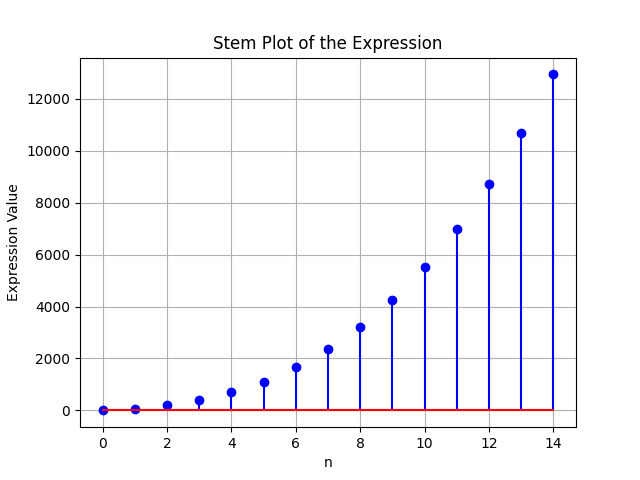
\includegraphics[width=\columnwidth]{images/plot.png}

        
            
           
             
             
             
        

        













\renewcommand{\thefigure}{\theenumi}
\renewcommand{\thetable}{\theenumi}





\end{document}
